\documentclass[10pt, a4paper]{jsarticle}
\usepackage[top=25truemm,bottom=25truemm,left=25truemm,right=25truemm]{geometry}
\usepackage{amsmath}
\usepackage{amsfonts}
\usepackage{courier}
\usepackage{here}
\usepackage[dvipdfmx]{graphicx}
\usepackage[ipaex]{pxchfon}
\newcommand{\1}{\mbox{1}\hspace{-0.25em}\mbox{l}}
\setlength{\columnsep}{3zw} 
\title{サンプルドキュメント} 
\author{{\bf furikake}\\{\small example}}
\date{}

\begin{document}
\maketitle

\section{概要}

これは概要である.

\section{実装}
\subsection{手法}

この自動ビルドシステムは\cite{ci}を参考にして作られている.

\begin{figure}[htbp]
  \centering
  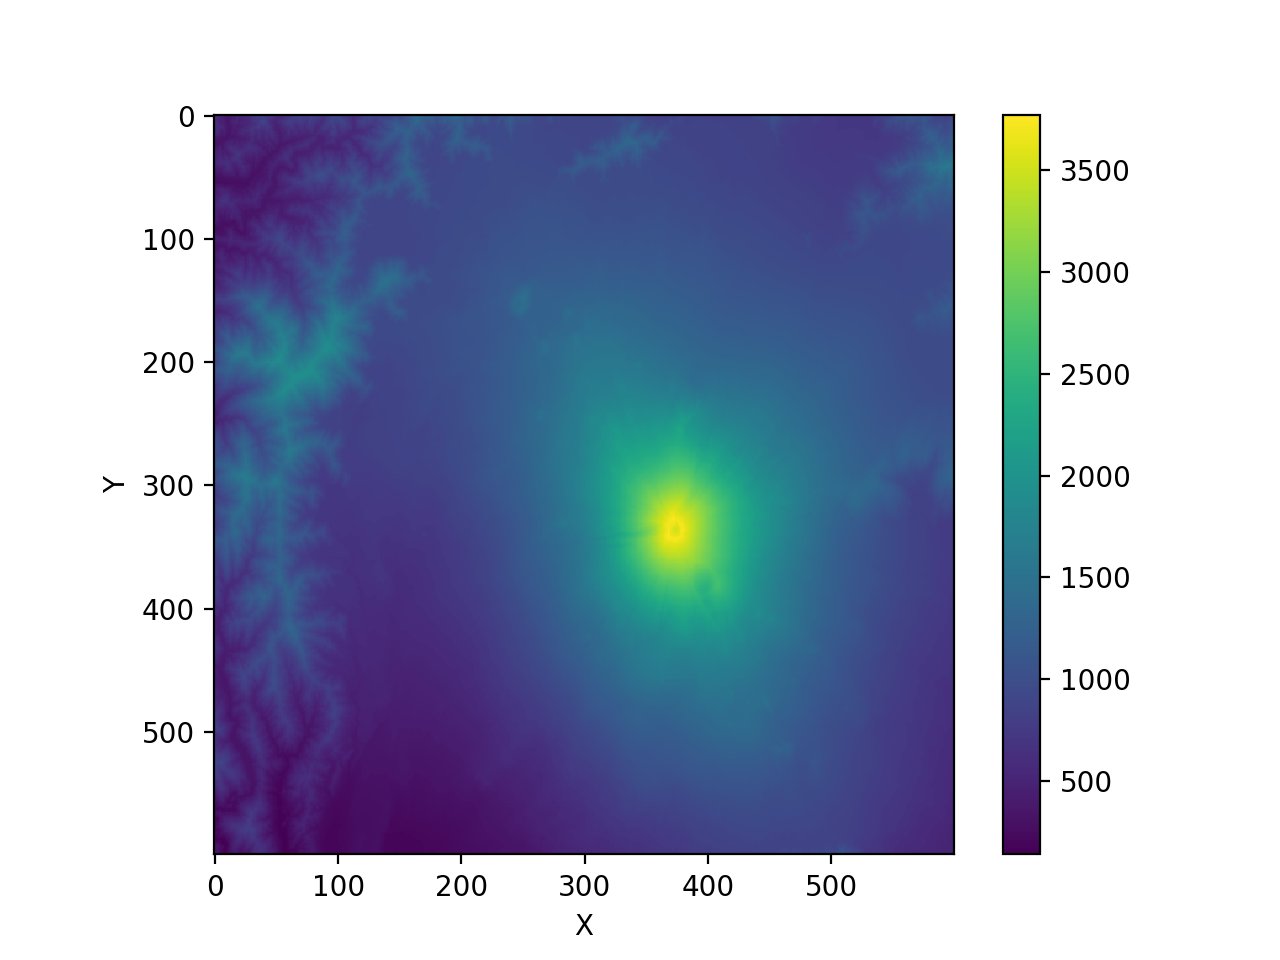
\includegraphics[width=10cm]{Figure_1.png}
  \caption{色分けグラフ}
  \label{fig: 2dcolor}
\end{figure}

\section{結論}

これは結論である.

\newpage
\bibliography{ref}
\bibliographystyle{junsrt}

\end{document}